\documentclass[fleqn,10pt]{wlscirep}
\usepackage[utf8]{inputenc}
\usepackage[T1]{fontenc}
\usepackage{caption}
\usepackage{subcaption}

\usepackage{hyperref}


\hypersetup{
    colorlinks=true,
    linkcolor=blue,
    filecolor=magenta,      
    urlcolor=cyan,
}
\usepackage{amsmath} % or simply amstext
\newcommand{\angstrom}{\text{\normalfont\AA}}

\title{A novel nucleoside-enzyme pair for stringent cell-specific metabolic labeling of RNA}

\author[1]{Sarah Nainar}
\author[1]{Bonnie Cuthbert}
\author[1]{Nathan M. Lim}
\author[1]{David L. Mobley}
\author[1]{Celia Goulding}
\author[1, *]{Robert Spitale}
\affil[1]{Department of Pharmaceutical Sciences, University of California---Irvine, Irvine, California 92697, United States}

\affil[*]{rspitale@uci.edu}

\begin{abstract}
    Abstract here.
\end{abstract}

\begin{document}

\flushbottom
\maketitle
\tableofcontents

\section{Computational Methods}
The starting structure used for the molecular dynamics (MD) simulations was taken from the crystal structure of human uridine-cytidine kinase 2 complex with the cytidine substrate (PDBID: 1UEJ) \cite{suzuki2004structural}.
In this study four different MD simulations were carried out, using two different binding modes for each of the respective ligands 2AZU and 2AZC.
Here, we differentiate between the two binding modes by the orientation of the ribose moiety on the molecule. 
The "canonical" binding mode refers to the pose in which the azide (substituted on the 2' position) is pointed inwards into the binding site, see Figure \ref{fig:2AZC-xtal}.
We refer to this as the canonical binding mode as this pose is similar to the pose found in the crystal structure with the bound cytidine substrate (PDBID: 1UEJ).
The "flipped" binding mode refer to the pose in which the azide is pointed outwards from the binding site, see Figure \ref{fig:2AZU-xtal}.

A total of 500ns of MD simulation time was conducted for each binding mode by running 5 simulations each, where each copy of the simulation began from the same protein structure.
The metastable binding modes sampled during our MD simulations were defined by constructing a Markov State Model (MSM) from our pool of MD simulation data and clustering with perron-cluster cluster analysis (PCCA).
We then compared these metastable binding modes with x-ray crystal structures for 2AZU and 2AZC by computing the root-mean-square deviation (RMSD) between the ligand heavy atoms.
We would like to note that the x-ray crystal structures of 2AZU and 2AZC were not used for setup or seen prior to conducting our MD simulations.
Our simulation results, along with the x-ray crystal structures, support the hypothesis that the ligands must adopt the "flipped" binding mode for catalytic turnover.

\subsection{Setup}
\subsubsection{MD simulation parameters}
All simulations in this study were conducted using OpenMM v7.1.1 \cite{openmm} at T=300K and P=1atm.
Here, we use timesteps of 4fs by employing the hydrogen mass repartitioning (HMR) scheme \cite{hmr}. 
This scheme allows us to take larger timesteps by slowing down the fastest motions (i.e. hydrogen bond stretching) in our MD simulations.
The HMR scheme constraints the bond length between hydrogens and their connected heavy atoms and reallocates mass from the connected heavy atom to the hydrogens.
The protein-ligand systems were placed in a periodic box with explicit TIP3P water molecules using a 10A solvent padding distance and counter ions (NaCl) were added using a concentration of 150mM.
A 10A cut-off distance was used for the particle-mesh Ewald method for computing long-range (e.g. electrostatic) interactions.
Protein atoms were parameterized using the `amber99sbildn' forcefields \cite{amber99sbildn} and the ligands were parameterized using GAFF2 \cite{ambergaff} in which atomic charges were assigned using the AM1-BCC charge model \cite{am1bcc}.

\subsubsection{Protein preparation}
To prepare the protein system (PDBID: 1UEJ) for MD simulations, we used PDBFixer \cite{pdbfixer} to model in missing residues, add missing hydrogen atoms, and solvate our system.
Sidechains were protonated in accordance with the pH=8.0 environment of the enzyme assay experiments \cite{doi:10.1021/bi102054n} and as described in other computational studies \cite{tanaka2016molecular}.
With the cytidine molecule bound, we energy minimized the protein-ligand complex for a maximum of 30,000 steps and followed with an equilibration protocol as follows.
The equilibration protocol occurs in four 10 ps stages, whereby a progressively declining restraining force was used to help the protein-ligand system gradually relax.
First, we apply a restraining force of 2.0 to the heavy atoms of the protein-ligand complex, simulate for 10ps using constant volume (NVT), and follow-up with 10ps at constant pressure (NPT).
Next, we decrease the restraining force to 0.5 and then conduct an NPT simulation for 10ps.
Last, we use a 0.1 restraining force on the alpha-carbons (protein backbone) and the ligand heavy atoms and then NPT simulate for 10ps.

\subsubsection{Docking}
After equilibration of the UCK2-cytidine complex, we applied HYBRID docking \cite{mcgann2012fred} to dock our nucleoside analogs (2AZU and 2AZC) into the binding site.
HYBRID differs from the standard docking approach such that the software will use the co-crystallized ligand as a reference point and attempt to fit the nucleoside analogs within the binding site by overlaying the docked ligands with the crystallographic ligand.
From HYBRID docking, we generated up to 50 different conformers for each nucleoside analog and then followed the same equilibration protocol described previously.
After equilibration, we found that the conformers tended to converge into two groups: 1 conformer which resembled the "canonical" binding mode and another which had the ribose moiety "flipped".
We then selected 1 conformer from each representative group and carried these forward for our production NPT 100ns MD simulations (no restraints).

\subsection{Analysis}
For each nuceloside analog (2AZC and 2AZU), we ran five 100ns MD simulations for each of the two binding modes (canonical and flipped).
They are denoted as $2AZC_{canc}$, $2AZC_{flip}$, $2AZU_{canc}$, and $2AZU_{flip}$.
Collectively, over the course of the 100ns of simulation time, the root-mean-square deviation (RMSD) for the ligand atoms began to stabilize after 25ns.
Thus, we discard trajectory frames from 0-25ns as additional equilibration time and only perform further analysis from the 25ns-100ns time frame Fig.\ref{fig:2AZC_canc-rmsd_trim}.
The RMSD is calculated by:
\begin{equation}
    RMSD = \sqrt{ \frac{1}{n} \sum^{n}_{i=1}{d_{i}^{2}}}
\end{equation}
where $d_{i}$ represents the distance between the $n$ atom pairs.
For construction of our Markov State models (MSM), we use the PyEMMA v2.5.5 \cite{scherer2015pyemma} toolkit.
For residue contact analyses we use the MDTraj v1.9.1 \cite{mcgibbon2015mdtraj} and VMD v1.9.3 \cite{humphrey1996vmd} toolkits.

\subsubsection{Defining the metastable binding modes}

\begin{figure}[!ht]
\centering
\begin{subfigure}{.5\textwidth}
  \centering
  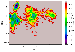
\includegraphics[width=.9\linewidth]{2AZC_canc/2AZC_canc-tica}
  \caption{$2AZC_{canc}-pcca$}
  \label{fig:2AZC_canc-tica}
\end{subfigure}%
\begin{subfigure}{.5\textwidth}
  \centering
  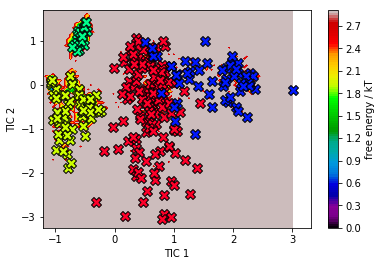
\includegraphics[width=.9\linewidth]{2AZC_canc/2AZC_canc-pcca}
  \caption{$2AZC_{canc}-pcca$}
  \label{fig:2AZC_canc-pcca}
\end{subfigure}
\caption{Caption for this figure with two images}
\label{fig:2AZC_canc-cluster}
\end{figure}

In order to define our metastable binding modes and visualize their structures, we construct a Markov State model (MSM) \cite{prinz2011markov} from our five separate MD simulations.
Our features for constructing the MSMs consists of the distance between the closest heavy atoms on the ligand and the following 9 residues: ASP62, PHE83, ASP84, TYR112, PHE114, HIS117, ILE137, ARG166, and ARG176.
These residues were selected as they have been noted in the literature to play important roles in binding \cite{tanaka2016molecular}.
From this feature space, we apply the time-lagged independent component analysis (TICA) method using a lagtime of 1ns.
TICA transforms our 9 dimensional feature space to a new set of reaction coordinates which maximizes the autocorrelation of the transformed coordinates \cite{perez2013identification}.
In other words, TICA allows us to extract the slow order parameters and project them into a lower dimensional space; here, we use the first two TICA coordinates (Fig. \ref{fig:2AZC_canc-tica}).
Then, we apply k-means clustering to discretize our trajectory frames into discrete microstate and project them into TICA space (denoted by individual Xs).
Following, we use perron-cluster cluster analysis (PCCA) \cite{roblitz2013fuzzy} to assign each microstate to a metastable macrostate (denoted by color in Fig.\ref{fig:2AZC_canc-pcca}).
From each of our assigned macrostates, we randomly sample 100 frames and then visualize the frame which minimizes the RMSD to the crystallographic ligand.

\subsubsection{Distance to key residues}
Using the `$compute\_contacts$' tool from MDTraj, we compute the distance between the closest heavy atoms in the ligand and 4 residues: ASP62, TYR112, HIS117 and ARG176 (Fig.\ref{fig:contact-distance}).
These residues were chosen in particular as ASP62 is known to be the catalytic residue, while TYR112, HIS117, and ARG176 are believed to play a key role in substrate specificity between uridine and cytidine as they have been found to bind to the nucleobase moiety \cite{tanaka2016molecular}.
Here, we calculate the frequency in which the distance between the ligand and the residues are less than or equal to 3.0A, which we define as the minimum distance needed to form an interactive bond.

\subsubsection{Hydrogen Bond Contacts}

We compute the frequency of hydrogen bond contacts between the ligands and surrounding residues using the HBonds plugin v1.2 in VMD 1.9.3 \cite{humphrey1996vmd}, shown in Figure \ref{fig:HBonds}.
The criterion used for defining formation of a hydrogen bond is that the cutoff distance between a hydrogen bond donor and acceptor must be less than 3.0\angstrom and the angle is less than 20 degrees.
Each colored bar corresponds to the hydrogen bond frequency from an individual MD simulation.

\subsubsection{Comparisons to X-ray Crystal Structures}
Here, we compared our metastable binding modes from our MD simulations against each subunit found in the experimental x-ray crystal structures and list the values against the subunit which minimizes the computed RMSD.
To compare the metastable binding modes from our MD simulations with experimental x-ray crystal structures, we first align the two structures using the protein backbone.
Particularly, we align by the protein backbone using residues 19 to 229 but exclude residues 48 to 52 as these were missing in the x-ray crystal structures.
Once aligned by the protein backbone, we then compute the RMSD between crystallized ligand and the matching ligand heavy atoms from our defined metastable binding modes.

\section{Results}

\subsection{Binding Mode Stability}

\begin{figure}[!ht]
\centering
   \begin{subfigure}{.45\textwidth}
     \centering
     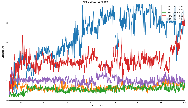
\includegraphics[width=.95\linewidth]{2AZC_canc/2AZC_canc-rmsd-trim}
     \caption{$2AZC_{canc}-rmsd_trim$}
     \label{fig:2AZC_canc-rmsd_trim}
   \end{subfigure}
   \begin{subfigure}{.45\textwidth}
     \centering
     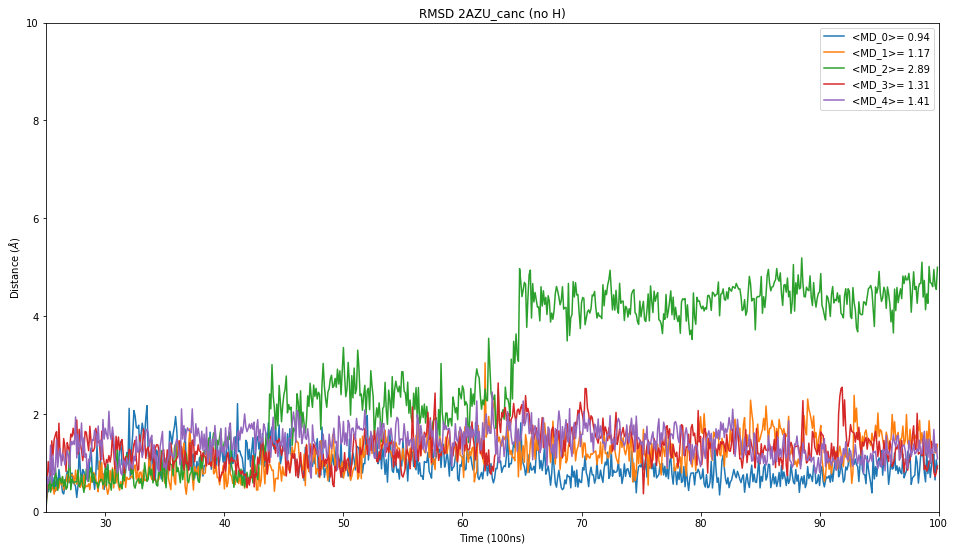
\includegraphics[width=.95\linewidth]{2AZU_canc/2AZU_canc-rmsd-trim}
     \caption{$2AZU_{canc}-rmsd_trim$}
     \label{fig:2AZU_canc-rmsd_trim}
   \end{subfigure}
   \\
   \begin{subfigure}{.45\textwidth}
     \centering
     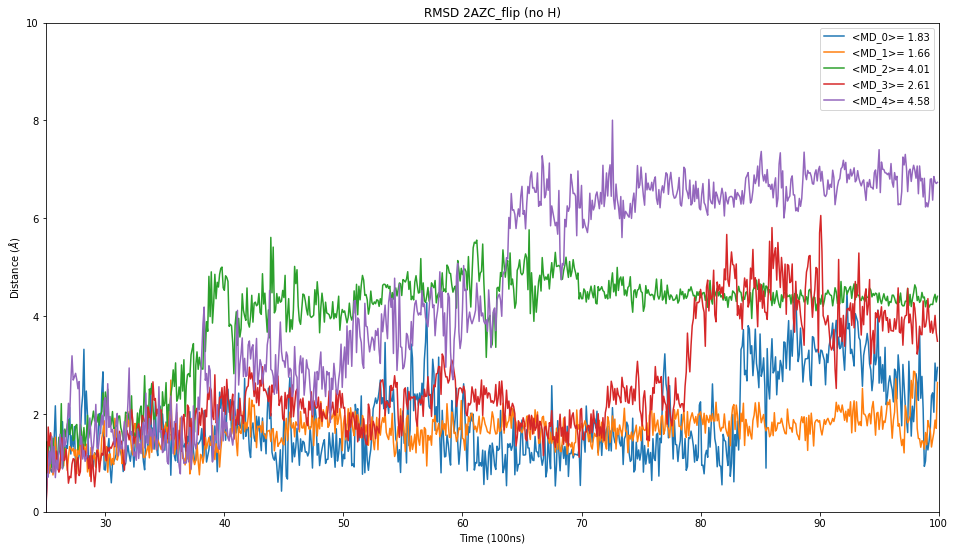
\includegraphics[width=.95\linewidth]{2AZC_flip/2AZC_flip-rmsd-trim}
     \caption{$2AZC_{flip}-rmsd_trim$}
     \label{fig:2AZC_flip-rmsd_trim}
   \end{subfigure}
    \begin{subfigure}{.45\textwidth}
     \centering
     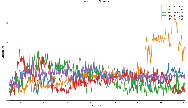
\includegraphics[width=.95\linewidth]{2AZU_flip/2AZU_flip-rmsd-trim}
     \caption{$2AZU_{flip}-rmsd_trim$}
     \label{fig:2AZU_flip-rmsd_trim}
   \end{subfigure}
\caption{Calculated RMSDs for ligand heavy atoms from 25-100ns MD simulations}
\label{fig:rmsd}
\end{figure}  

\begin{table}[!ht]
\caption{Calculated RMSDs for ligand heavy atoms from 25-100ns MD simulations}
\label{table:rmsd}
\begin{tabular}{|l|l|l|l|l|l|l|l|}
\hline
                    & RMSD & RMSD & RMSD & RMSD & RMSD & \textbf{AVG}  & SEM           \\ \hline
\textbf{2AZC\_canc} & 6.66 & 1.36 & 1.14 & 4.12 & 2.06 & \textbf{3.07} & \textit{1.04} \\ \hline
\textbf{2AZU\_canc} & 0.94 & 1.17 & 2.89 & 1.31 & 1.41 & \textbf{1.54} & \textit{0.35} \\ \hline
\textbf{2AZC\_flip} & 1.83 & 1.66 & 4.01 & 2.61 & 4.58 & \textbf{2.94} & \textit{0.58} \\ \hline
\textbf{2AZU\_flip} & 2.43 & 3.08 & 2.35 & 2.23 & 2.61 & \textbf{2.54} & \textit{0.15} \\ \hline

\end{tabular}
\end{table}

The averages and the standard errors of the mean (SEM) for the RMSD of each ligand binding mode are shown in Fig.\ref{fig:rmsd} and Table\ref{table:rmsd}.
They are $3.07 \frac{+}{-} 1.04$, $1.54 \frac{+}{-} 0.35$, $2.94 \frac{+}{-} 0.58$, and $2.54 \frac{+}{-} 0.15$ for $2AZC_{canc}$, $2AZU_{canc}$, $2AZC_{flip}$, and $2AZU_{flip}$, respectively.

Comparing the RMSD of the cannonical binding modes for 2AZC and 2AZU, we find that the 2AZU ligand to be much more stable than the 2AZC ligand.
In $\frac{2}{5}$ of our MD simulations for $2AZC_{canc}$ (Fig.\ref{fig:2AZC_canc-rmsd_trim}), the ligand comes nearly unbound after 30ns; while for $2AZU_{canc}$ (Fig. \ref{fig:2AZU_canc-rmsd_trim}) the ligand nearly unbinds in only $\frac{1}{5}$ of the simulations.
When comparing $2AZC_{flip}$ and $2AZU_{flip}$, the average RMSD suggests both are about equally stable.
However, this particular binding mode appears to show slightly more instability than the cannonical binding mode with an average RMSD of $2.54$ and $2.94$ for the $2AZC_{flip}$ and $2AZU_{flip}$, respectively.

\subsubsection{Distance to key residues}

In Figure \ref{fig:contact-distance}, we plot the distance between the closest ligand heavy atoms and the 4 residues: ASP62 (blue), TYR112 (orange), HIS117 (green) and ARG176 (red).
One plot from each respective binding mode was chosen from the simulation in which contact with the catalytic residue ASP62 was highest.
Additional plots from the other MD simulations for binding modes can be found in the supporting information.
See Figure \ref{sup:2AZC_canc-dist} for $2AZC_{canc}$, Figure \ref{sup:2AZU_canc-dist} for $2AZU_{canc}$, Figure \ref{sup:2AZC_flip-dist} for $2AZC_{flip}$, and Figure \ref{sup:2AZU_flip-dist} for $2AZU_{flip}$.

For the canonical binding mode, we see a maximum contact frequency of 3.9\% (2AZC) and 2.5\% (2AZU) in which the ligand is $d<3.0\angstrom$ away from the catalytic residue ASP62.
Figure \ref{fig:2AZC_canc-dist} shows that the 2AZC ligand in the canonical binding mode only rarely comes into contact with ASP62 but is in stable contact with HIS117 and ARG176.  
Interestingly, Figure \ref{fig:2AZU_canc-dist} illustrates that even though the ligand appears to be stably bound to the key residues (TYR112, HIS117, and ARG176) the ligand may be too far away from ASP62 for catalysis.

In stark contrast, we see an enormous increase in contact frequency when simulating the flipped binding mode; 27.9\% (2AZC) and 80.4\% (2AZU).
Figure \ref{fig:2AZC_flip-dist} shows the 2AZC ligand forms stable contacts with the catalytic residue ASP62 and residues TYR112/HIS117 but does not contact ARG176.
Similarly, we see the same stable contacts being formed for 2AZU in Figure \ref{fig:2AZU_flip-dist}.

These results suggest that the canonical binding mode may not be the binding mode the ligand adopts for catalytic turnover.
Instead, our results indicate that the ligand must adopt the flipped conformation and that contact with residues TYR112/HIS117 appear to be necessary for catalytic turnover.
Here, residue ARG176 seems to only serves a role in stabilizing the ligand in the binding site when in the canonical conformation.
We believe the canonical conformation may represent the post-catalytic binding mode and ARG176 plays a role in the post-catalytic process.
From Figure \ref{sup:2AZC_flip-dist}, there are several moments when the ligand $2AZC_{flip}$ comes into closer contact with ARG176, the distance with ASP62 increases and vice versa.

\begin{figure}[!ht]
\centering
   \begin{subfigure}{.45\textwidth}
     \centering
     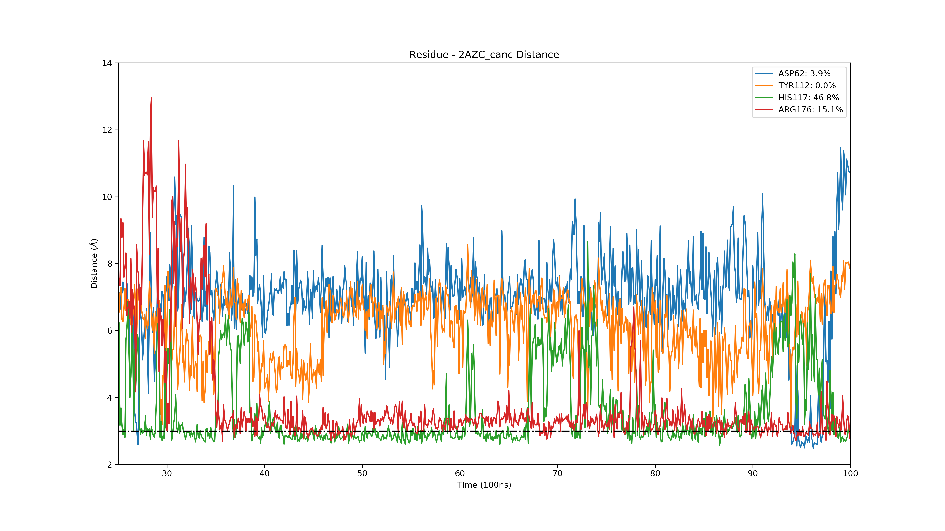
\includegraphics[width=.95\linewidth]{2AZC_canc/2AZC_canc-dist_3.pdf}
     \caption{$2AZC_{canc}-distance$}
     \label{fig:2AZC_canc-dist}
   \end{subfigure}
   \begin{subfigure}{.45\textwidth}
     \centering
     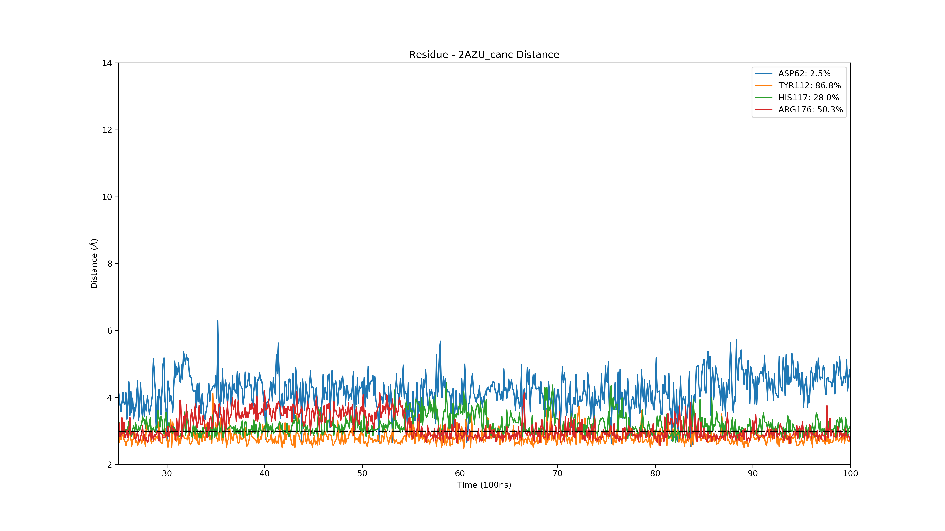
\includegraphics[width=.95\linewidth]{2AZU_canc/2AZU_canc-dist_4.pdf}
     \caption{$2AZU_{canc}-distance$}
     \label{fig:2AZU_canc-dist}
   \end{subfigure}
   \\
   \begin{subfigure}{.45\textwidth}
     \centering
     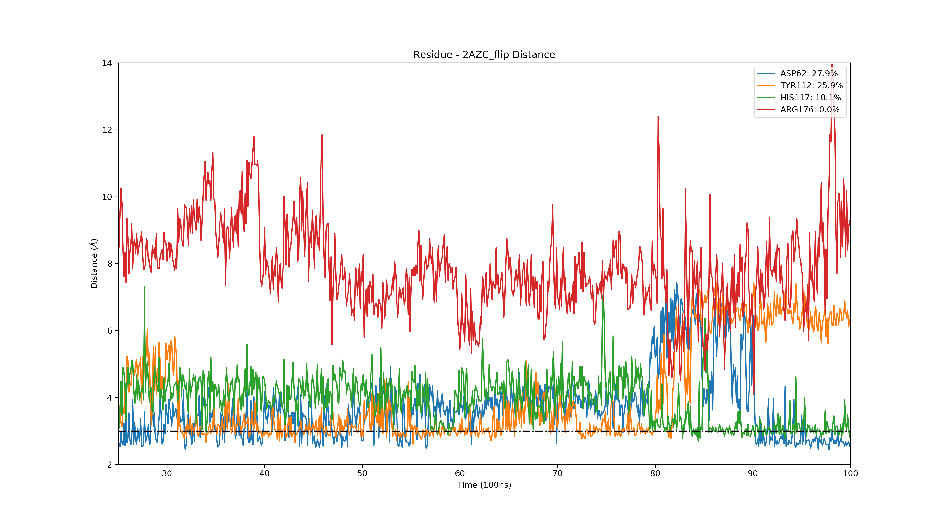
\includegraphics[width=.95\linewidth]{2AZC_flip/2AZC_flip-dist_3.pdf}
     \caption{$2AZC_{flip}-distance$}
     \label{fig:2AZC_flip-dist}
   \end{subfigure}
    \begin{subfigure}{.45\textwidth}
     \centering
     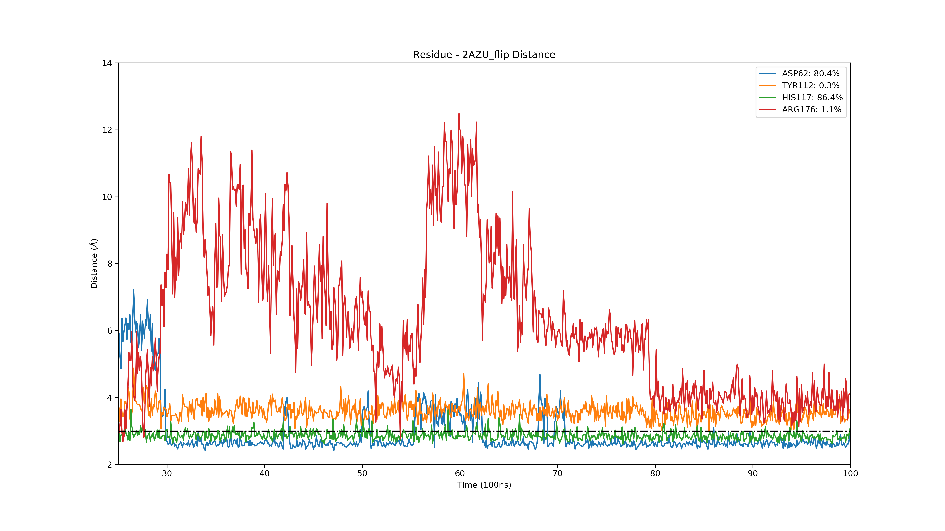
\includegraphics[width=.95\linewidth]{2AZU_flip/2AZU_flip-dist_4.pdf}
     \caption{$2AZU_{flip}-distance$}
     \label{fig:2AZU_flip-dist}
   \end{subfigure}
\caption{contact-distance}
\label{fig:contact-distance}
\end{figure}  

\subsubsection{Hydrogen Bond Contacts}

\begin{figure}[!ht]
\centering
   \begin{subfigure}{.45\textwidth}
     \centering
     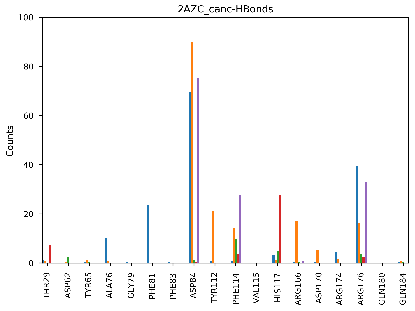
\includegraphics[width=.95\linewidth]{2AZC_canc/2AZC_canc-HBonds.pdf}
     \caption{$2AZC_{canc}-HBonds$}
     \label{fig:2AZC_canc-HBonds}
   \end{subfigure}
   \begin{subfigure}{.45\textwidth}
     \centering
     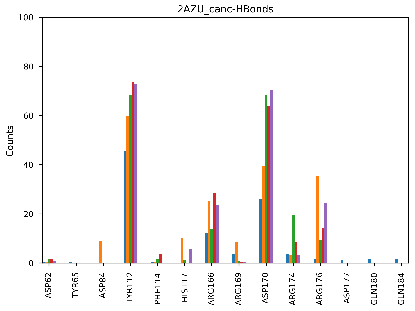
\includegraphics[width=.95\linewidth]{2AZU_canc/2AZU_canc-HBonds.pdf}
     \caption{$2AZU_{canc}-HBonds$}
     \label{fig:2AZU_canc-HBonds}
   \end{subfigure}
   \\
   \begin{subfigure}{.45\textwidth}
     \centering
     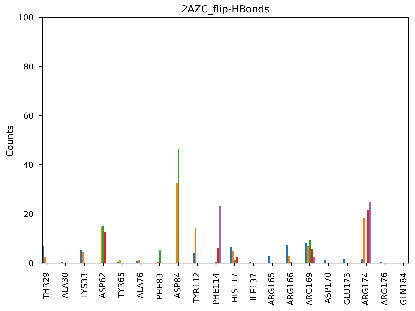
\includegraphics[width=.95\linewidth]{2AZC_flip/2AZC_flip-HBonds.pdf}
     \caption{$2AZC_{flip}-HBonds$}
     \label{fig:2AZC_flip-HBonds}
   \end{subfigure}
    \begin{subfigure}{.45\textwidth}
     \centering
     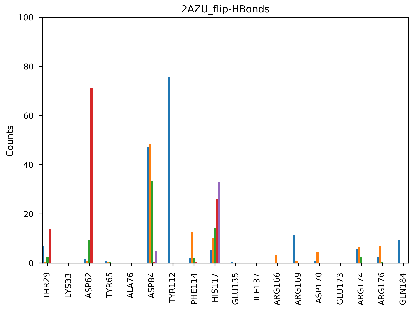
\includegraphics[width=.95\linewidth]{2AZU_flip/2AZU_flip-HBonds.pdf}
     \caption{$2AZU_{flip}-HBonds$}
     \label{fig:2AZU_flip-HBonds}
   \end{subfigure}
\caption{HBonds}
\label{fig:HBonds}
\end{figure}  

In order to gain some insight on the interactions required for catalysis, we profile the hydrogen bond contacts between the ligand and surrounding protein residues.
When comparing the cannonical binding modes, we see that $2AZC_{canc}$ forms hydrogen bond contacts mostly with ASP84, PHE114, HIS117, and ARG176; but no virtually no contact with the catalytic residue ASP62 (Fig. \ref{fig:2AZC_canc-HBonds}).
For $2AZU_{canc}$ (Fig. \ref{fig:2AZU_canc-HBonds}), we frequent contacts with TYR112, ARG166, ASP170, and ARG176; also, virtually no contact with the catalytic residue ASP62.
Given that we do not see hydrogen bonding between the ligand and ASP62, this supports the hypothesis that the canonical binding mode may not be the pose required for catalysis.

For the flipped binding mode, we see a much higher rate of contact to ASP62 which supports the hypothesis that this binding mode may be what the ligand adopts for catalytic turnover.
In Figure \ref{fig:2AZC_flip-HBonds}, we see ~20\% contact with ASP62 and moderate rates of contact with ASP84, PHE114, HIS117, ARG169, and ARG174.
For $2AZC_{flip}$, contact with ASP62 (yellow/green/red) appears to be related to hydrogen bonding with ASP84 (yellow/green), TYR112(yellow) and ARG174 (yellow).
In Figure \ref{fig:2AZU_flip-HBonds}, we see ~70\% contact with ASP62 and moderate contacts with THR29, ASP84, TYR112, and HIS117.
For $2AZU_{flip}$, contact with ASP62(green/red) appears to be related to hydrogen bonding with THR29(red), ASP84(green) and HIS117(green/red).

From our results, we hypothesize that ASP84 plays a critical role in binding the both substrates for catalysis, given that we see high rates of contact for both 2AZU and 2AZC.
The binding of 2AZC appears to specifically require contact with either ARG174/ARG176 residues and potentially contact with TYR112 for additional stability.
In contrast, binding of 2AZU with TYR112 does not appear to prepare the ligand for catalysis (based on the flipped binding mode) but appears to stabilize the binding mode post-catalysis (based on the cannonical binding mode).
For specificity of binding 2AZU, it appears that hydrogen bonding with HIS117 is required and potentially contact with THR29 for additional stability.

\subsubsection{Comparison to X-ray Crystal Structures}

\begin{figure}[!ht]
\centering
\begin{subfigure}{.5\textwidth}
  \centering
  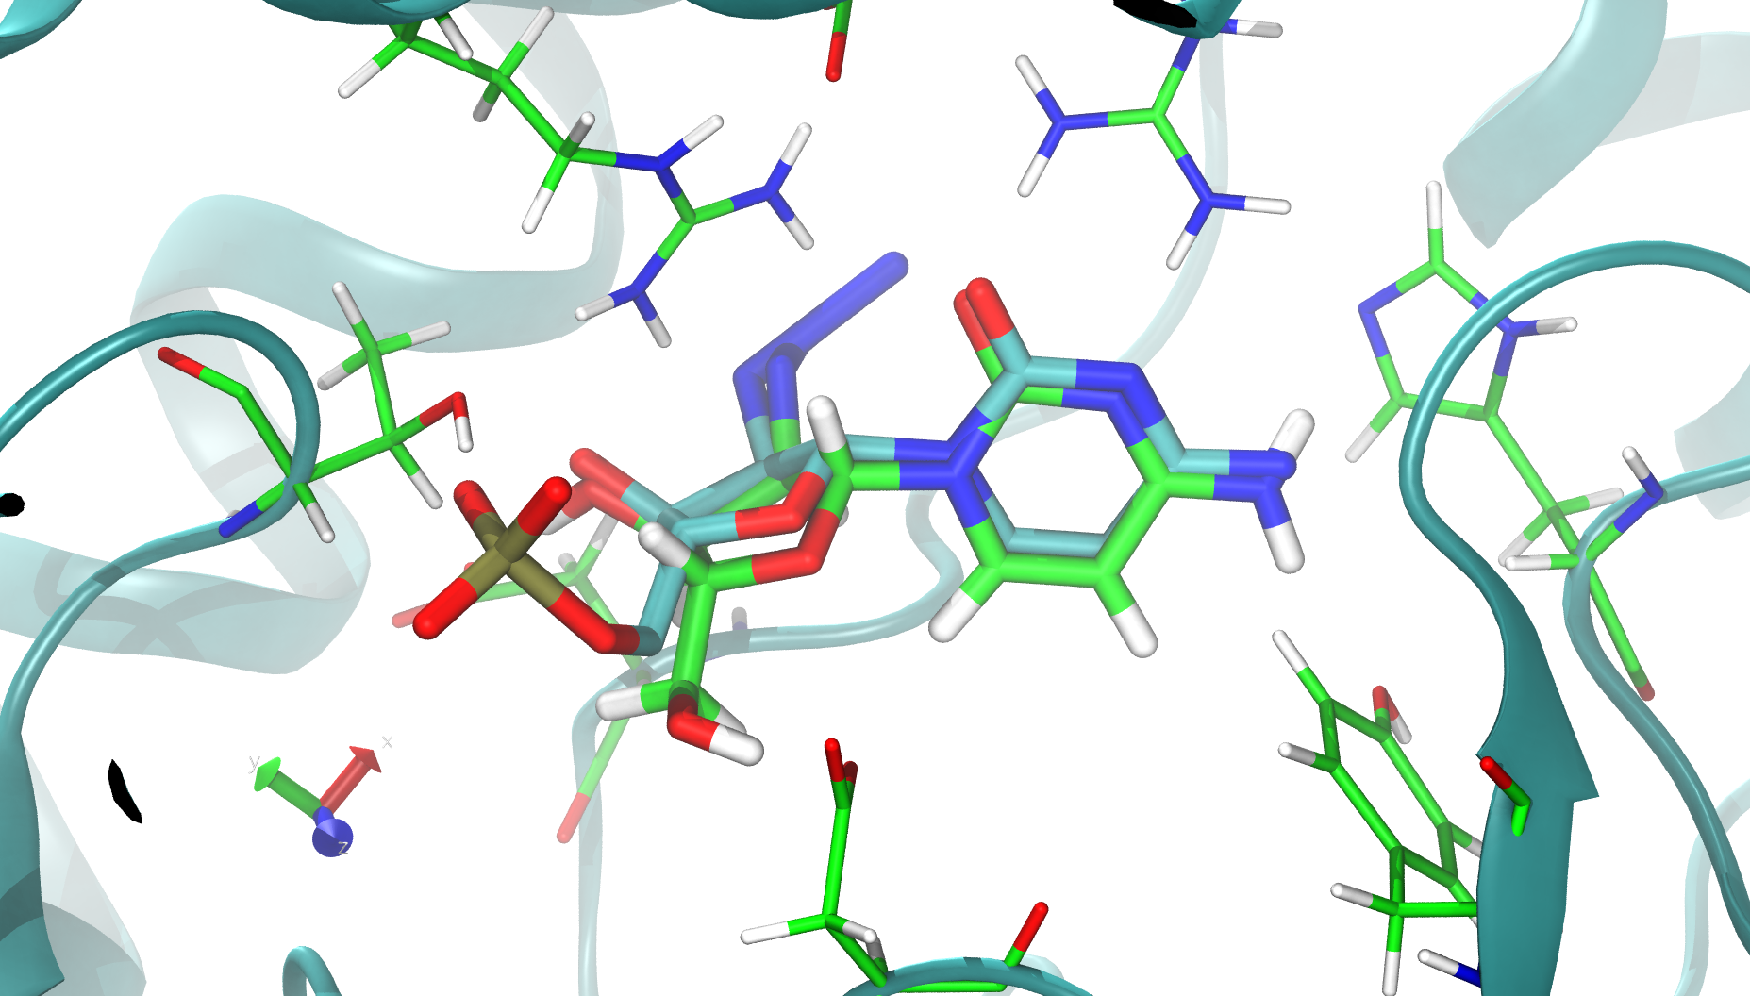
\includegraphics[width=.9\linewidth]{xtal/2AZC_canc-xtal_front.pdf}
  \caption{$2AZC_{canc}-xtal$}
  \label{fig:2AZC-xtal}
\end{subfigure}%
\begin{subfigure}{.5\textwidth}
  \centering
  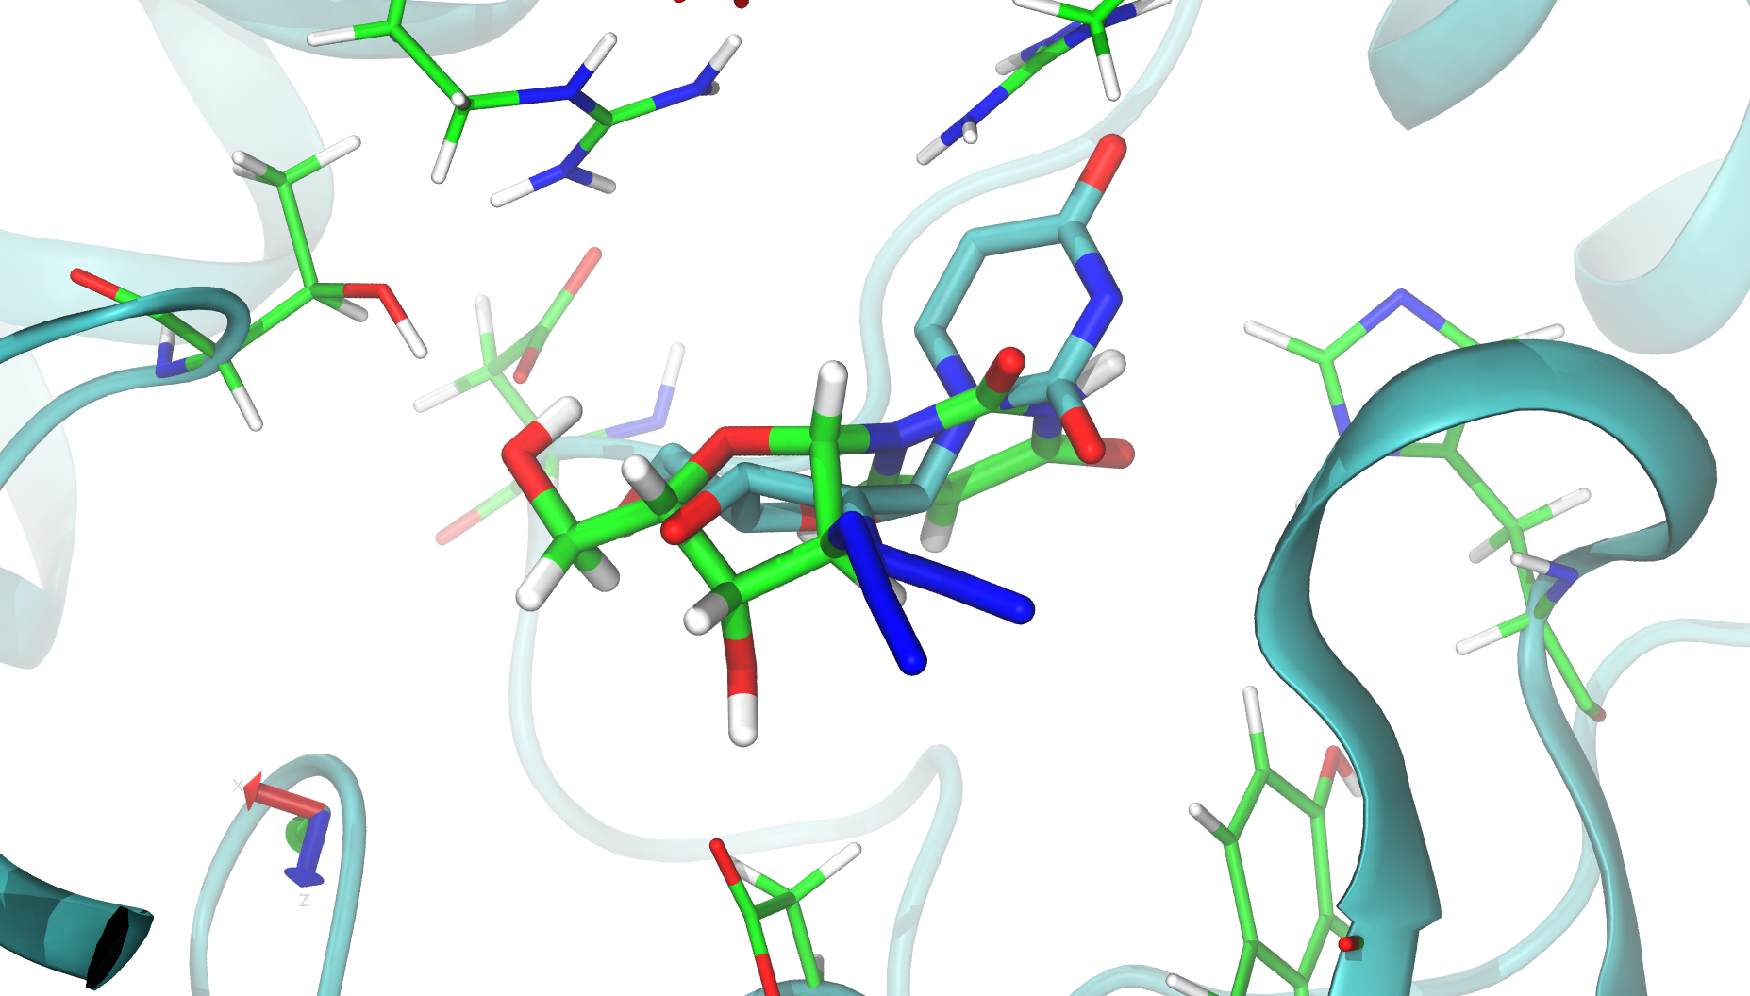
\includegraphics[width=.9\linewidth]{xtal/2AZU_flip-xtal_front.pdf}
  \caption{$2AZU_{flip}-xtal$}
  \label{fig:2AZU-xtal}
\end{subfigure}
\caption{Caption for this figure with two images}
\label{fig:xtal}
\end{figure}


\begin{table}[!ht]
\begin{tabular}{|l|l|l|}
\hline
                          & \textbf{$2AZC_{xtal}-A$} & \textbf{$BB_{RMSD}$} \\ \hline
\textbf{$2AZC_{canc}-pcca3$} & 0.72                  & 1.20             \\ \hline
\textbf{$2AZC_{flip}-pcca3$} & 5.04                  & 1.47              \\ \hline
\textbf{}                 & \textbf{$2AZU_{xtal}-F$} & \textbf{$BB_{RMSD}$} \\ \hline
\textbf{$2AZU_{canc}-pcca1$} & 4.84                  & 2.67             \\ \hline
\textbf{$2AZU_{flip}-pcca0$} & 2.31                  & 2.81              \\ \hline
\end{tabular}
\end{table}

Here, we compared our defined metastable binding modes from our MD simulations to our x-ray crystal structures by computing the RMSD between matching heavy atoms in the respective ligands.
The crystal structure containing the 2AZU ligand was found to bind similarly as the flipped binding mode from our MD simulation.
The minimum computed RMSD of $2AZU_{flip}$ from our MD simulation against the x-ray crystal structure was 2.31\angstrom; while for $2AZU_{canc}$ was 4.84\angstrom.
On the other hand, the crystal structure obtained for 2AZC was found to resemble the post-catalytic state, as the bound ligand contained an attached phosphate group.
The minimum computed RMSD of $2AZC_{canc}$ was 0.72\angstrom and was 5.04 for $2AZC_{flip}$.
These results provide strong supporting evidence that the flipped binding mode represents the conformer of the ligand before catalysis; while the canonical binding mode represents the post-catalytic state.

\section{Discussion}
%The Discussion should be succinct and must not contain subheadings.

Prior to running our MD simulations, we had no experimental evidence which suggests the existence of an alternative binding mode.
We first discovered the flipped binding mode after our HYBRID docking approach with our short equilibration protocol.
The x-ray crystal structure of 2AZC represents the system in it's post-catalytic state and has a phosphate group attached, thus we exclude the phosphate group from our RMSD calculations as our simulations represent the pre-catalytic state.
The x-ray crystal structure of 2AZU represents the system in it's pre-catalytic state and has no added phosphate group, so no atoms were excluded from the RMSD calculation.



\bibliography{references}

\section{Acknowledgements}

Christopher Bayly and Gaetano Calabro at OpenEye Scientific Software for development of the MD simulation protocol.

\section{Author contributions statement}

S.N. and R.S. conceived the experiment(s), S.N. conducted the experiment(s),  B.C crystallized the system, and N.M.L conducted the computational experiments.  All authors reviewed the manuscript. 

\section{Additional information}

\subsection{MSM and Clustering}

\begin{figure}[!ht]
\centering
\begin{subfigure}{.5\textwidth}
  \centering
  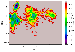
\includegraphics[width=.9\linewidth]{2AZC_canc/2AZC_canc-tica.pdf}
  \caption{$2AZC_{canc}-pcca$}
  \label{sup:2AZC_canc-tica}
\end{subfigure}%
\begin{subfigure}{.5\textwidth}
  \centering
  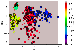
\includegraphics[width=.9\linewidth]{2AZC_canc/2AZC_canc-pcca.pdf}
  \caption{$2AZC_{canc}-pcca$}
  \label{sup:2AZC_canc-pcca}
\end{subfigure}
\caption{Caption for this figure with two images}
\label{sup:2AZC_canc-cluster}
\end{figure}

\begin{figure}[!ht]
\centering
\begin{subfigure}{.5\textwidth}
  \centering
  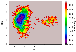
\includegraphics[width=.9\linewidth]{2AZU_canc/2AZU_canc-tica.pdf}
  \caption{$2AZU_{canc}-pcca$}
  \label{sup:2AZU_canc-tica}
\end{subfigure}%
\begin{subfigure}{.5\textwidth}
  \centering
  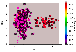
\includegraphics[width=.9\linewidth]{2AZU_canc/2AZU_canc-pcca.pdf}
  \caption{$2AZU_{canc}-pcca$}
  \label{sup:2AZU_canc-pcca}
\end{subfigure}
\caption{Caption for this figure with two images}
\label{sup:2AZU_canc-cluster}
\end{figure}

\begin{figure}[!ht]
\centering
\begin{subfigure}{.5\textwidth}
  \centering
  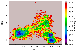
\includegraphics[width=.9\linewidth]{2AZC_flip/2AZC_flip-tica.pdf}
  \caption{$2AZC_{flip}-pcca$}
  \label{sup:2AZC_flip-tica}
\end{subfigure}%
\begin{subfigure}{.5\textwidth}
  \centering
  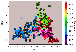
\includegraphics[width=.9\linewidth]{2AZC_flip/2AZC_flip-pcca.pdf}
  \caption{$2AZC_{flip}-pcca$}
  \label{sup:2AZC_flip-pcca}
\end{subfigure}
\caption{Caption for this figure with two images}
\label{sup:2AZC_flip-cluster}
\end{figure}

\begin{figure}[!ht]
\centering
\begin{subfigure}{.5\textwidth}
  \centering
  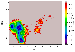
\includegraphics[width=.9\linewidth]{2AZU_flip/2AZU_flip-tica.pdf}
  \caption{$2AZU_{flip}-pcca$}
  \label{sup:2AZU_flip-tica}
\end{subfigure}%
\begin{subfigure}{.5\textwidth}
  \centering
  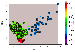
\includegraphics[width=.9\linewidth]{2AZU_flip/2AZU_flip-pcca.pdf}
  \caption{$2AZU_{flip}-pcca$}
  \label{sup:2AZU_flip-pcca}
\end{subfigure}
\caption{Caption for this figure with two images}
\label{sup:2AZU_flip-cluster}
\end{figure}


\subsection{Distance to key residues}

\begin{figure}[!ht]
\centering
  \begin{subfigure}{.45\textwidth}
     \centering
     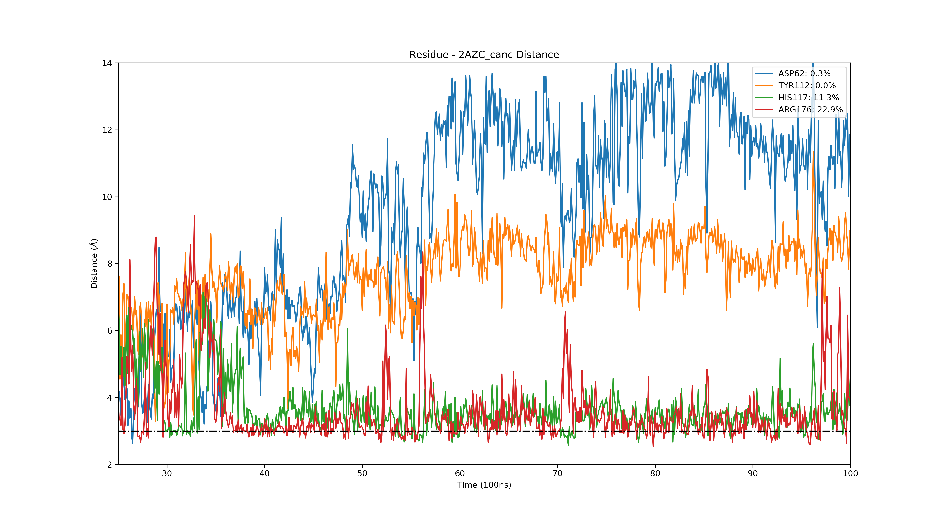
\includegraphics[width=.95\linewidth]{2AZC_canc/2AZC_canc-dist_0.pdf}
  \end{subfigure}
  \begin{subfigure}{.45\textwidth}
     \centering
     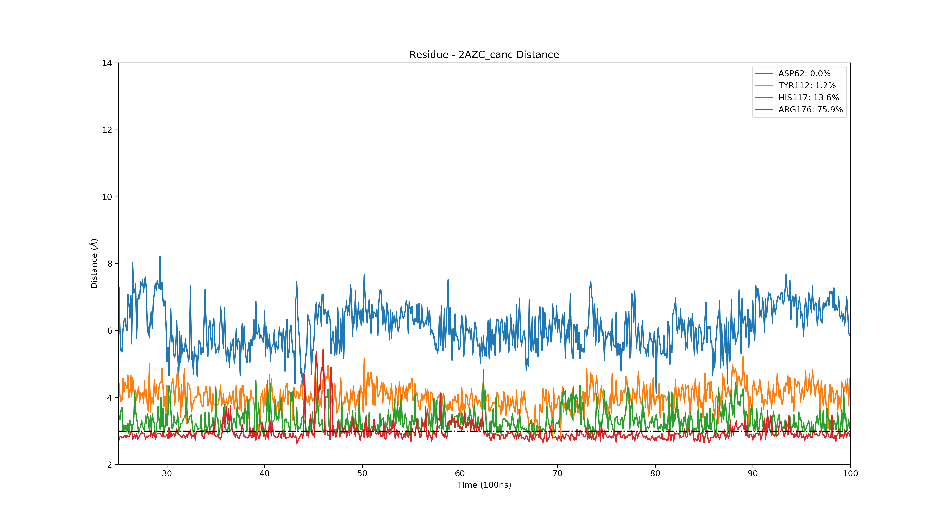
\includegraphics[width=.95\linewidth]{2AZC_canc/2AZC_canc-dist_1.pdf}
  \end{subfigure}
  \\
  \begin{subfigure}{.45\textwidth}
     \centering
     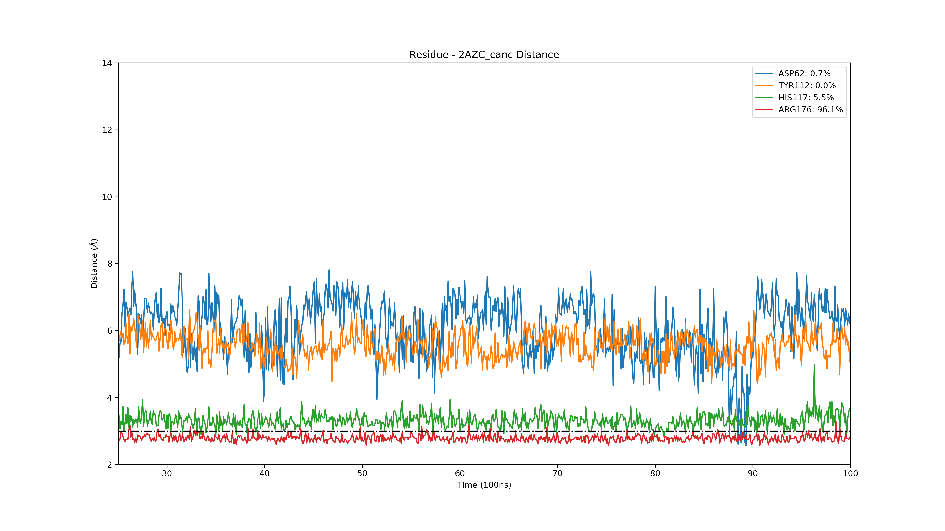
\includegraphics[width=.95\linewidth]{2AZC_canc/2AZC_canc-dist_2.pdf}
  \end{subfigure}
    \begin{subfigure}{.45\textwidth}
     \centering
     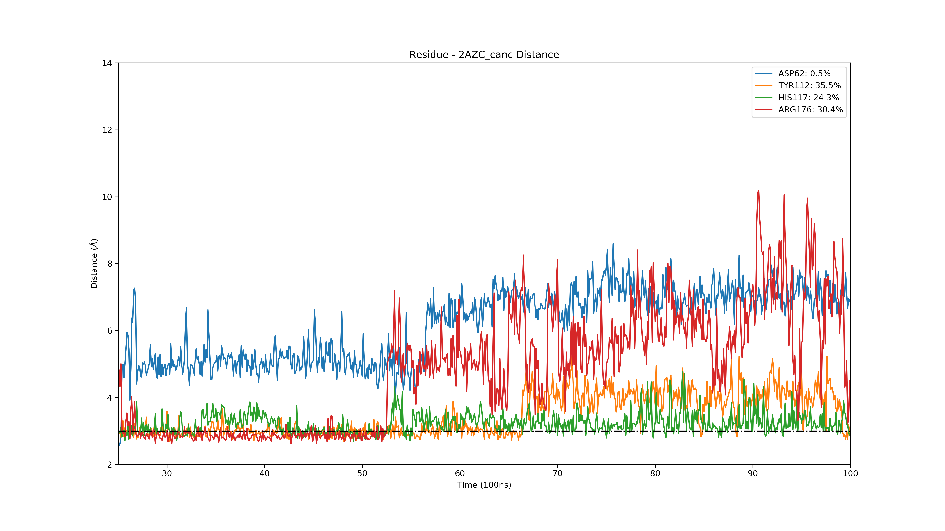
\includegraphics[width=.95\linewidth]{2AZC_canc/2AZC_canc-dist_4.pdf}
  \end{subfigure}
\caption{$2AZC_{canc}-distance$}
\label{sup:2AZC_canc-dist}
\end{figure}  


\begin{figure}[!ht]
\centering
  \begin{subfigure}{.45\textwidth}
     \centering
     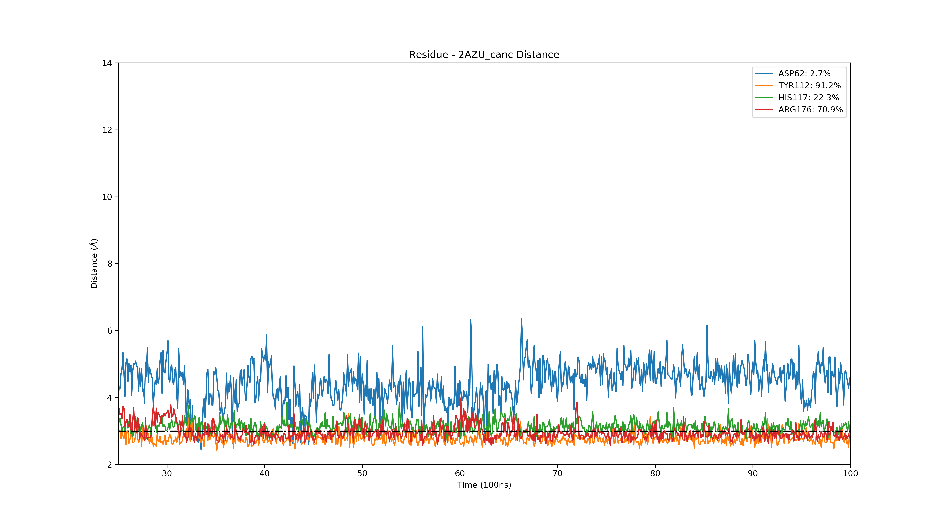
\includegraphics[width=.95\linewidth]{2AZU_canc/2AZU_canc-dist_0.pdf}
  \end{subfigure}
  \begin{subfigure}{.45\textwidth}
     \centering
     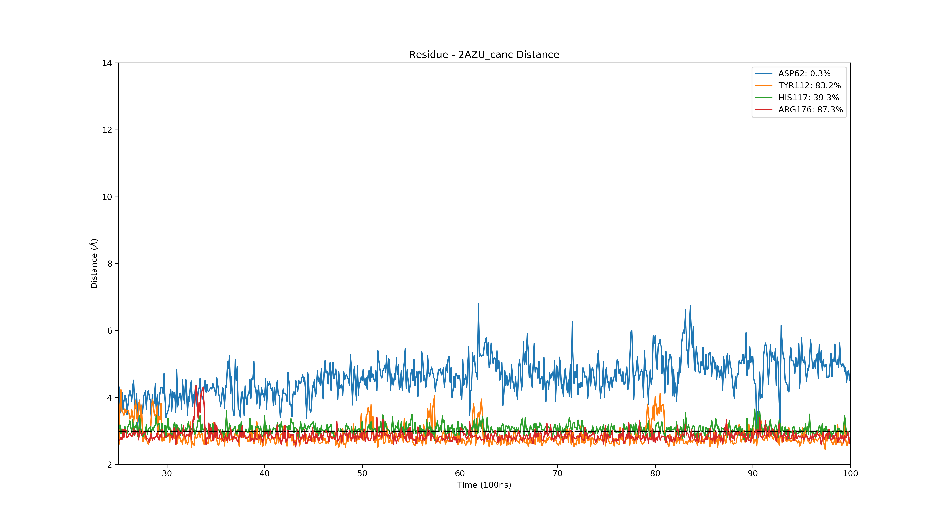
\includegraphics[width=.95\linewidth]{2AZU_canc/2AZU_canc-dist_1.pdf}
  \end{subfigure}
  \\
  \begin{subfigure}{.45\textwidth}
     \centering
     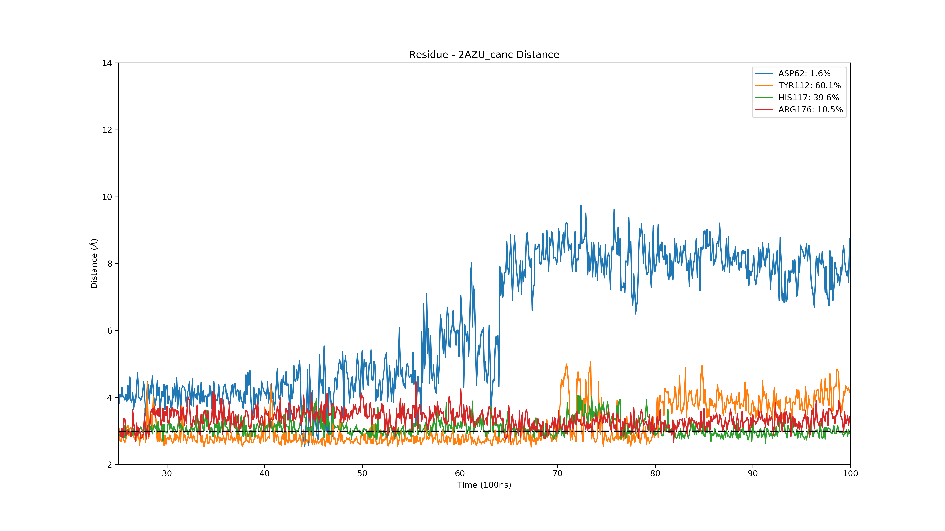
\includegraphics[width=.95\linewidth]{2AZU_canc/2AZU_canc-dist_2.pdf}
  \end{subfigure}
    \begin{subfigure}{.45\textwidth}
     \centering
     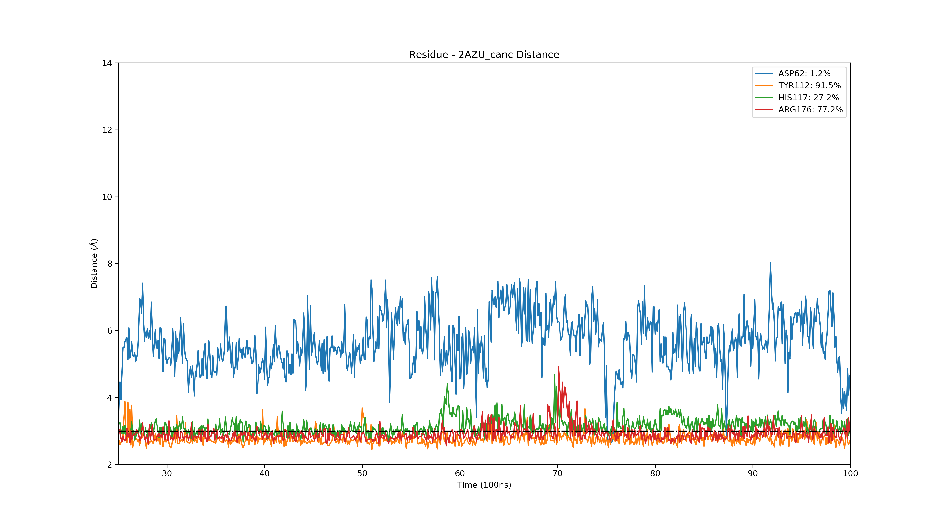
\includegraphics[width=.95\linewidth]{2AZU_canc/2AZU_canc-dist_3.pdf}
  \end{subfigure}
\caption{$2AZU_{canc}-distance$}
\label{sup:2AZU_canc-dist}
\end{figure}  

\begin{figure}[!ht]
\centering
  \begin{subfigure}{.45\textwidth}
     \centering
     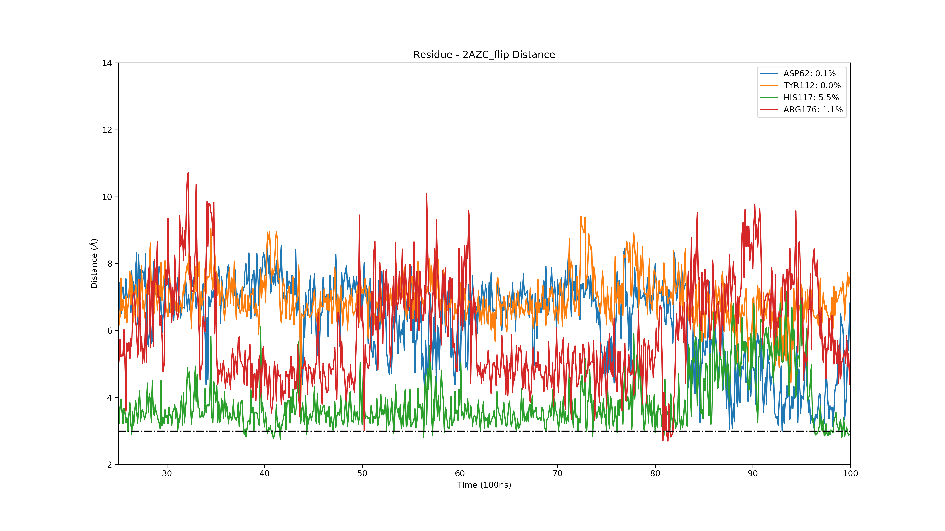
\includegraphics[width=.95\linewidth]{2AZC_flip/2AZC_flip-dist_0.pdf}
  \end{subfigure}
  \begin{subfigure}{.45\textwidth}
     \centering
     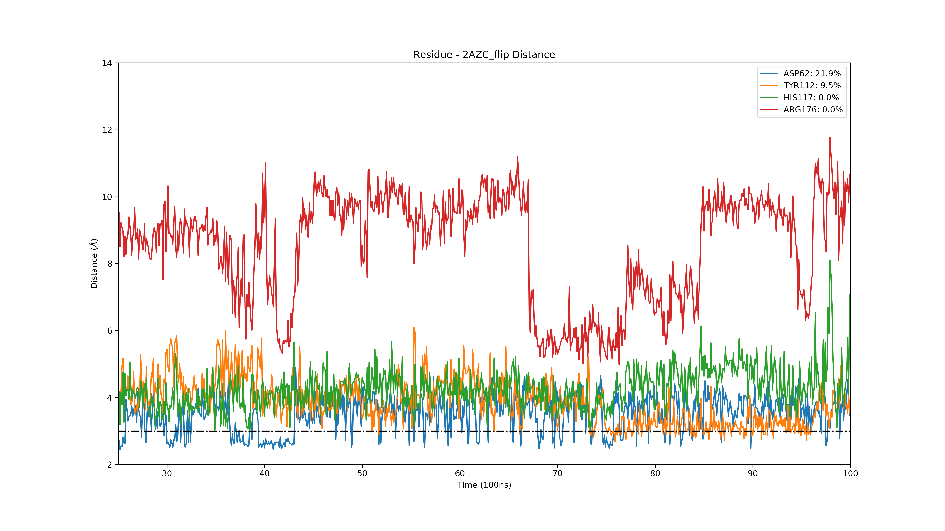
\includegraphics[width=.95\linewidth]{2AZC_flip/2AZC_flip-dist_1.pdf}
  \end{subfigure}
  \\
  \begin{subfigure}{.45\textwidth}
     \centering
     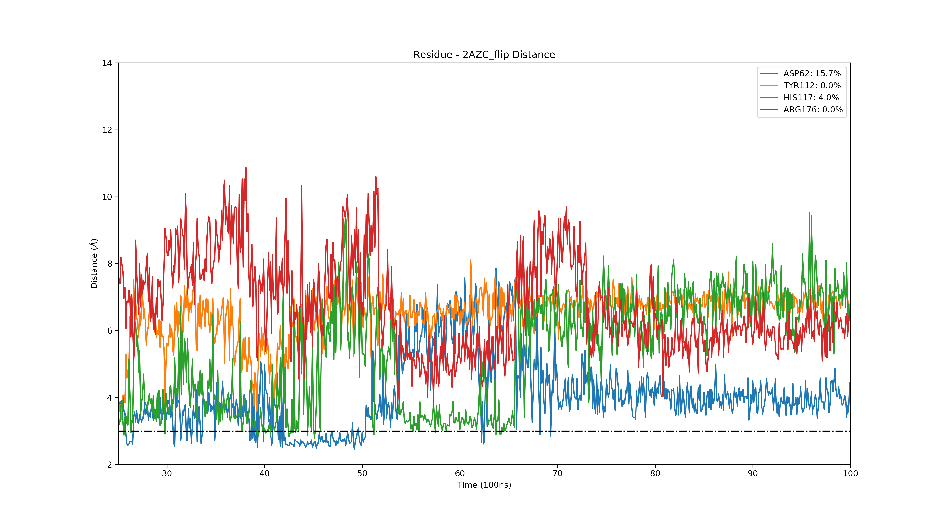
\includegraphics[width=.95\linewidth]{2AZC_flip/2AZC_flip-dist_2.pdf}
  \end{subfigure}
    \begin{subfigure}{.45\textwidth}
     \centering
     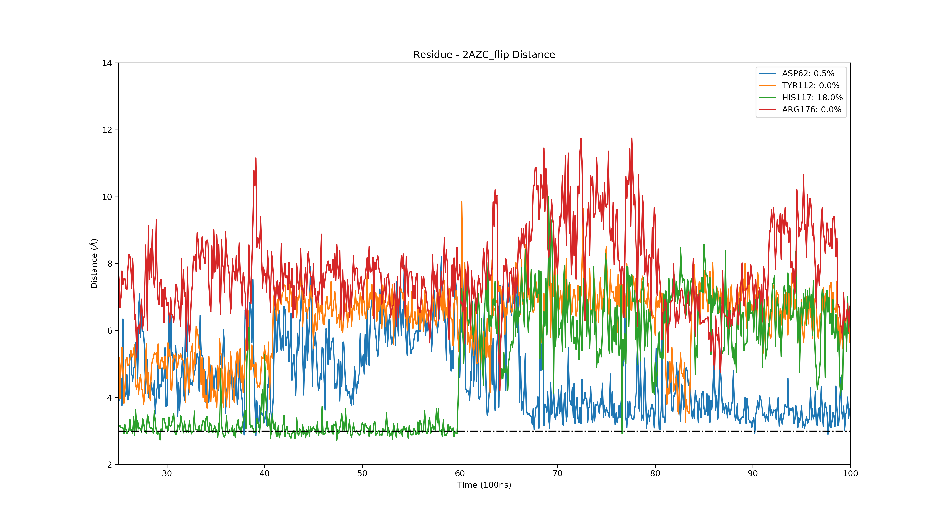
\includegraphics[width=.95\linewidth]{2AZC_flip/2AZC_flip-dist_4.pdf}
  \end{subfigure}
\caption{$2AZC_{flip}-distance$}
\label{sup:2AZC_flip-dist}
\end{figure}  

\begin{figure}[!ht]
\centering
  \begin{subfigure}{.45\textwidth}
     \centering
     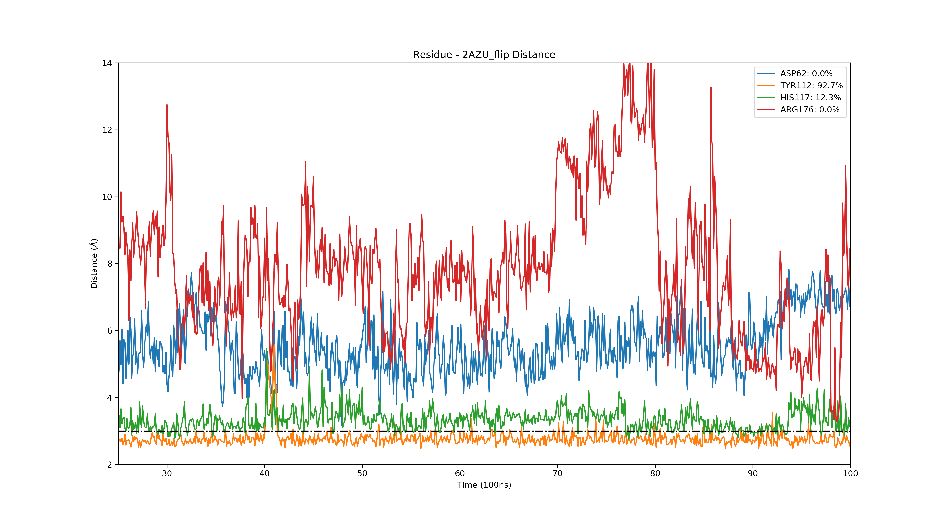
\includegraphics[width=.95\linewidth]{2AZU_flip/2AZU_flip-dist_0.pdf}
  \end{subfigure}
  \begin{subfigure}{.45\textwidth}
     \centering
     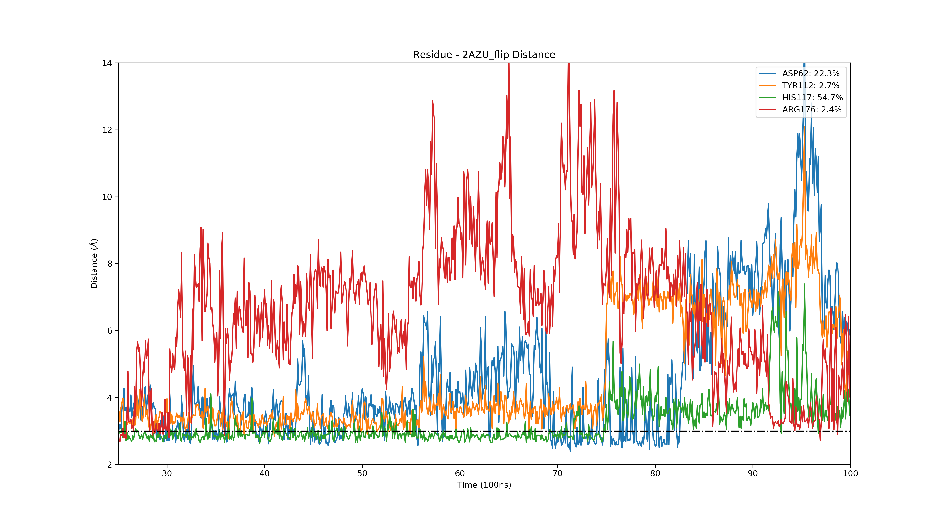
\includegraphics[width=.95\linewidth]{2AZU_flip/2AZU_flip-dist_1.pdf}
  \end{subfigure}
  \\
  \begin{subfigure}{.45\textwidth}
     \centering
     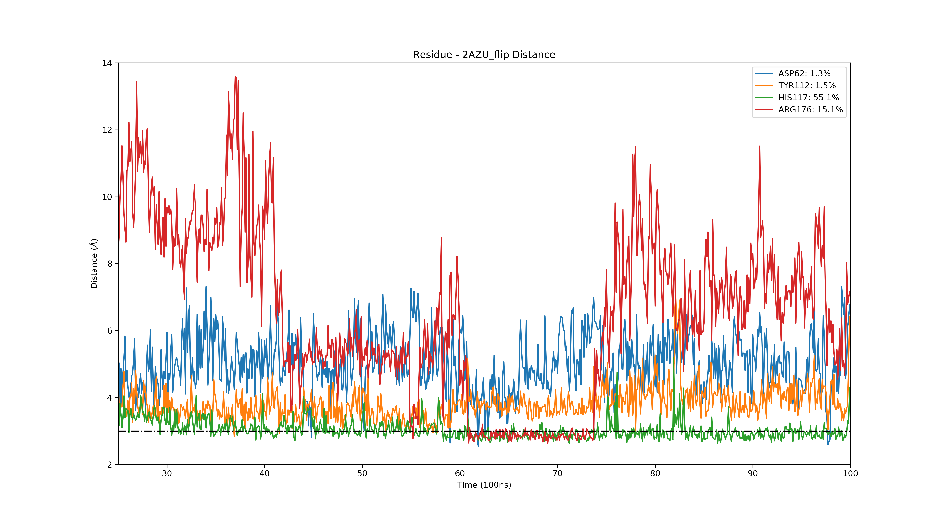
\includegraphics[width=.95\linewidth]{2AZU_flip/2AZU_flip-dist_2.pdf}
  \end{subfigure}
    \begin{subfigure}{.45\textwidth}
     \centering
     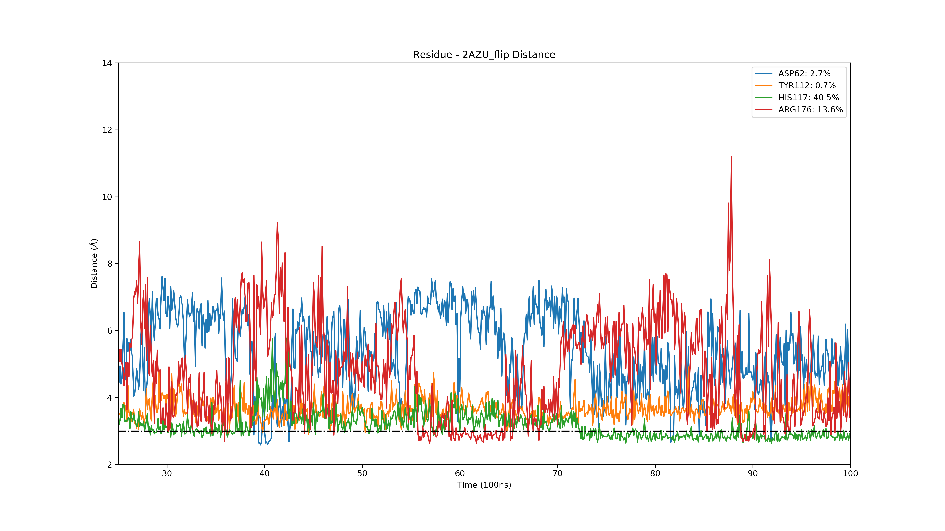
\includegraphics[width=.95\linewidth]{2AZU_flip/2AZU_flip-dist_3.pdf}
  \end{subfigure}
\caption{$2AZU_{flip}-distance$}
\label{sup:2AZU_flip-dist}
\end{figure}  

\end{document}